\documentclass[../Draft_harmonization_paper.tex]{subfiles}
% \documentclass{article}
% \usepackage[utf8]{inputenc}
% \usepackage{hyperref}
% \usepackage{float}
% \usepackage[table,xcdraw]{xcolor}
% \usepackage{color, colortbl}
% \usepackage{longtable}
% %\usepackage[sort&compress,square,comma,authoryear]{natbib}
% \usepackage{booktabs}
% \usepackage{graphicx}
% \graphicspath{{/home/kunz/Dokumente/Projects/Trait_DB/Invertebrate_traits/Paper/Figures/}}
% \usepackage{longtable}
% \usepackage{rotating}
% \usepackage{geometry}
% \usepackage{array}

% \definecolor{Gray}{gray}{0.9}

% \newcommand{\specialcell}[2][c]{%
%   \begin{tabular}[#1]{@{}c@{}}#2\end{tabular}}

\begin{document}

\section{Description of trait aggregation methods}

Traits of the harmonized grouping feature databases were aggregated to family-level using three approaches. I) we directly aggregated taxa to family-level giving equal weight to every species. We denote this aggregation as \textit{direct\_agg}. For the \textit{direct\_agg} we tested aggregating with the median and the mean. We added \textit{median} or \textit{mean} to \textit{direct\_agg} to indicate when we used which method. II) taxa were aggregated stepwise, i.e first to the genus-level and subsequently to the family-level. By using this approach, we give equal weights to each genus. Hereafter, we abbreviate this aggregation type as \textit{stepwise\_agg}.
We tested the \textit{stepwise\_agg} using the mean and the median, using the same naming as for the \textit{direct\_agg}. III) taxa were aggregated using a weighted mean approach, denoted as \textit{weighted\_agg}. The weights were determined as the ratio of the number of species per genera. This method weights the genera according to the number of their species present in the databases.

Trait affinities ranged between 0 and 1. Hence, the maximum differences possible is 1 or -1 (corresponds to 100 \%). For convenience, we report absolute trait differences.

% TODO: Mention usage of terminology from Schmera et al
%%%%%%%%%%%%%%%%%%%%%%%%%%%%%%%%%%%%%%%%%%%%%%%%%%%%%%%%%%%%%%%%%%%%%%%%%%%%%%%%%%%%%%%%%%%%%%%%%%%
%%%%%%%%%%%%%%%%%%%%%%%%%%%%%%%%%%%%%%%%%%%%%%%%%%%%%%%%%%%%%%%%%%%%%%%%%%%%%%%%%%%%%%%%%%%%%%%%%%%
\section{Differences in trait affinities obtained by trait aggregation methods compared to traits assigned at family-level}
\label{sec:diff_trait_agg_chessman}

Aggregated trait affinities using five trait aggregation methods (\textit{direct\_agg (median)}, \textit{direct\_agg (mean)}, \textit{stepwise\_agg (median)}, \textit{stepwise\_agg (mean)} and \textit{weighted\_agg}) were compared to trait affinities assigned at family-level by experts, which were available for the Australian and North American database for a limited subset of grouping features and taxa. For the Australian database, we compared aggregated trait affinities with assigned trait affinities resolved at family-level for the grouping features feeding mode and size by using data from Chessman 2018 (\cite{chessman_dissolved-oxygen_2018}). We could carry out the comparison to all taxa available in Chessman 2018, which contained trait information for 220 families. Considering each factor combination of family and investigated trait this amounts to 1760 cases. For the North American database, we compared aggregated trait affinities with assigned trait affinities on family-level for the grouping features feeding mode, respiration, size, voltinism, and locomotion from Pyne et al. Trait information in the Pyne et al database was available on the categorical scale and was converted to binary traits prior to the comparison with aggregated trait affinities. Trait information on family-level in the Pyne et al. database was available for 94 families of which all were present in the aggregated North American database (total number of cases 1598).

The percentage of differing cases of trait affinities obtained by the trait aggregation methods compared to trait affinities assigned at family-level varied between 16.18 \% and 22.9 \% for the Australian database. For the North American database, comparison of the trait aggregation methods to trait affinities assigned at family-level yielded between 15.3 \% and 47 \% differing cases (Table \ref{tab:summary_stat_aggr_vs_fam_assigned}).

For both databases maximum differences of 1 occurred for all investigated grouping features (Figure \ref{fig:diff_aggr_traits_chessman} and Figure \ref{fig:diff_aggr_traits_pyne}). In general, trait aggregation methods using the median yielded less cases with differences compared to approaches using the mean. However, using the median produced greater differences for both databases. 
% For the North American database the mean of absolute differences for the \textit{direct\_agg (median)} was more than twice 
% Mention taxa groups with many differing cases?

% TODO: Sidewaystable?
\begin{table}[H]
  \centering
  \caption{Amount of differing cases, the minimum and maximum, and means and standard deviations of absolute differences between trait affinities assigned at family-level and aggregated trait affinities.}
  \label{tab:summary_stat_aggr_vs_fam_assigned}
  \begin{tabular}{ll|ccccc}
  \hline
  Database & \specialcell{Comparison to\\ traits at fam.-lvl.} & \specialcell{Differing \\ cases [\%]} & \specialcell{Min. \\ differences} & \specialcell{Max. \\ differences} & \specialcell{Mean abs. \\ differences} & \specialcell{SD abs. \\ differences} \\ 
  \hline
  \multirow{4}{*}{\specialcell{Australia \\ (Chessman)}} & \specialcell{direct\_agg (median)} & 16.53 & 0.01 & 1.00 & 0.45 & 0.27 \\ 
  & \specialcell{direct\_agg (mean)} & 23.24 & $< 0.01$ & 0.99 & 0.34 & 0.23 \\ 
  & \specialcell{stepwise\_agg (median)} & 17.90 & 0.01 & 1.00 & 0.42 & 0.26 \\ 
  & \specialcell{stepwise\_agg (mean)} & 23.24 & $< 0.01$ & 0.99 & 0.33 & 0.22 \\ 
  & \specialcell{weighted\_agg} & 23.24 & $< 0.01$ & 1.00 & 0.34 & 0.24 \\ 
  \hline
  \multirow{4}{*}{\specialcell{North America \\ (Pyne)}} & \specialcell{direct\_agg (median)} & 15.33 & 0.17 & 1.00 & 0.70 & 0.26 \\ 
  & \specialcell{direct\_agg (mean)} & 47.00 & $< 0.01$ & 1.00 & 0.30 & 0.26 \\ 
  & \specialcell{stepwise\_agg (median)} & 18.00 & 0.08 & 1.00 & 0.63 & 0.28 \\ 
  & \specialcell{stepwise\_agg (mean)} & 47.00 & $< 0.01$ & 1.00 & 0.30 & 0.27 \\ 
  & \specialcell{weighted\_agg} & 47.00 & $< 0.01$ & 1.00 & 0.31 & 0.28 \\ 
  \hline
  \end{tabular}
\end{table}

\newpage

\begin{figure}[H]
  \centering
  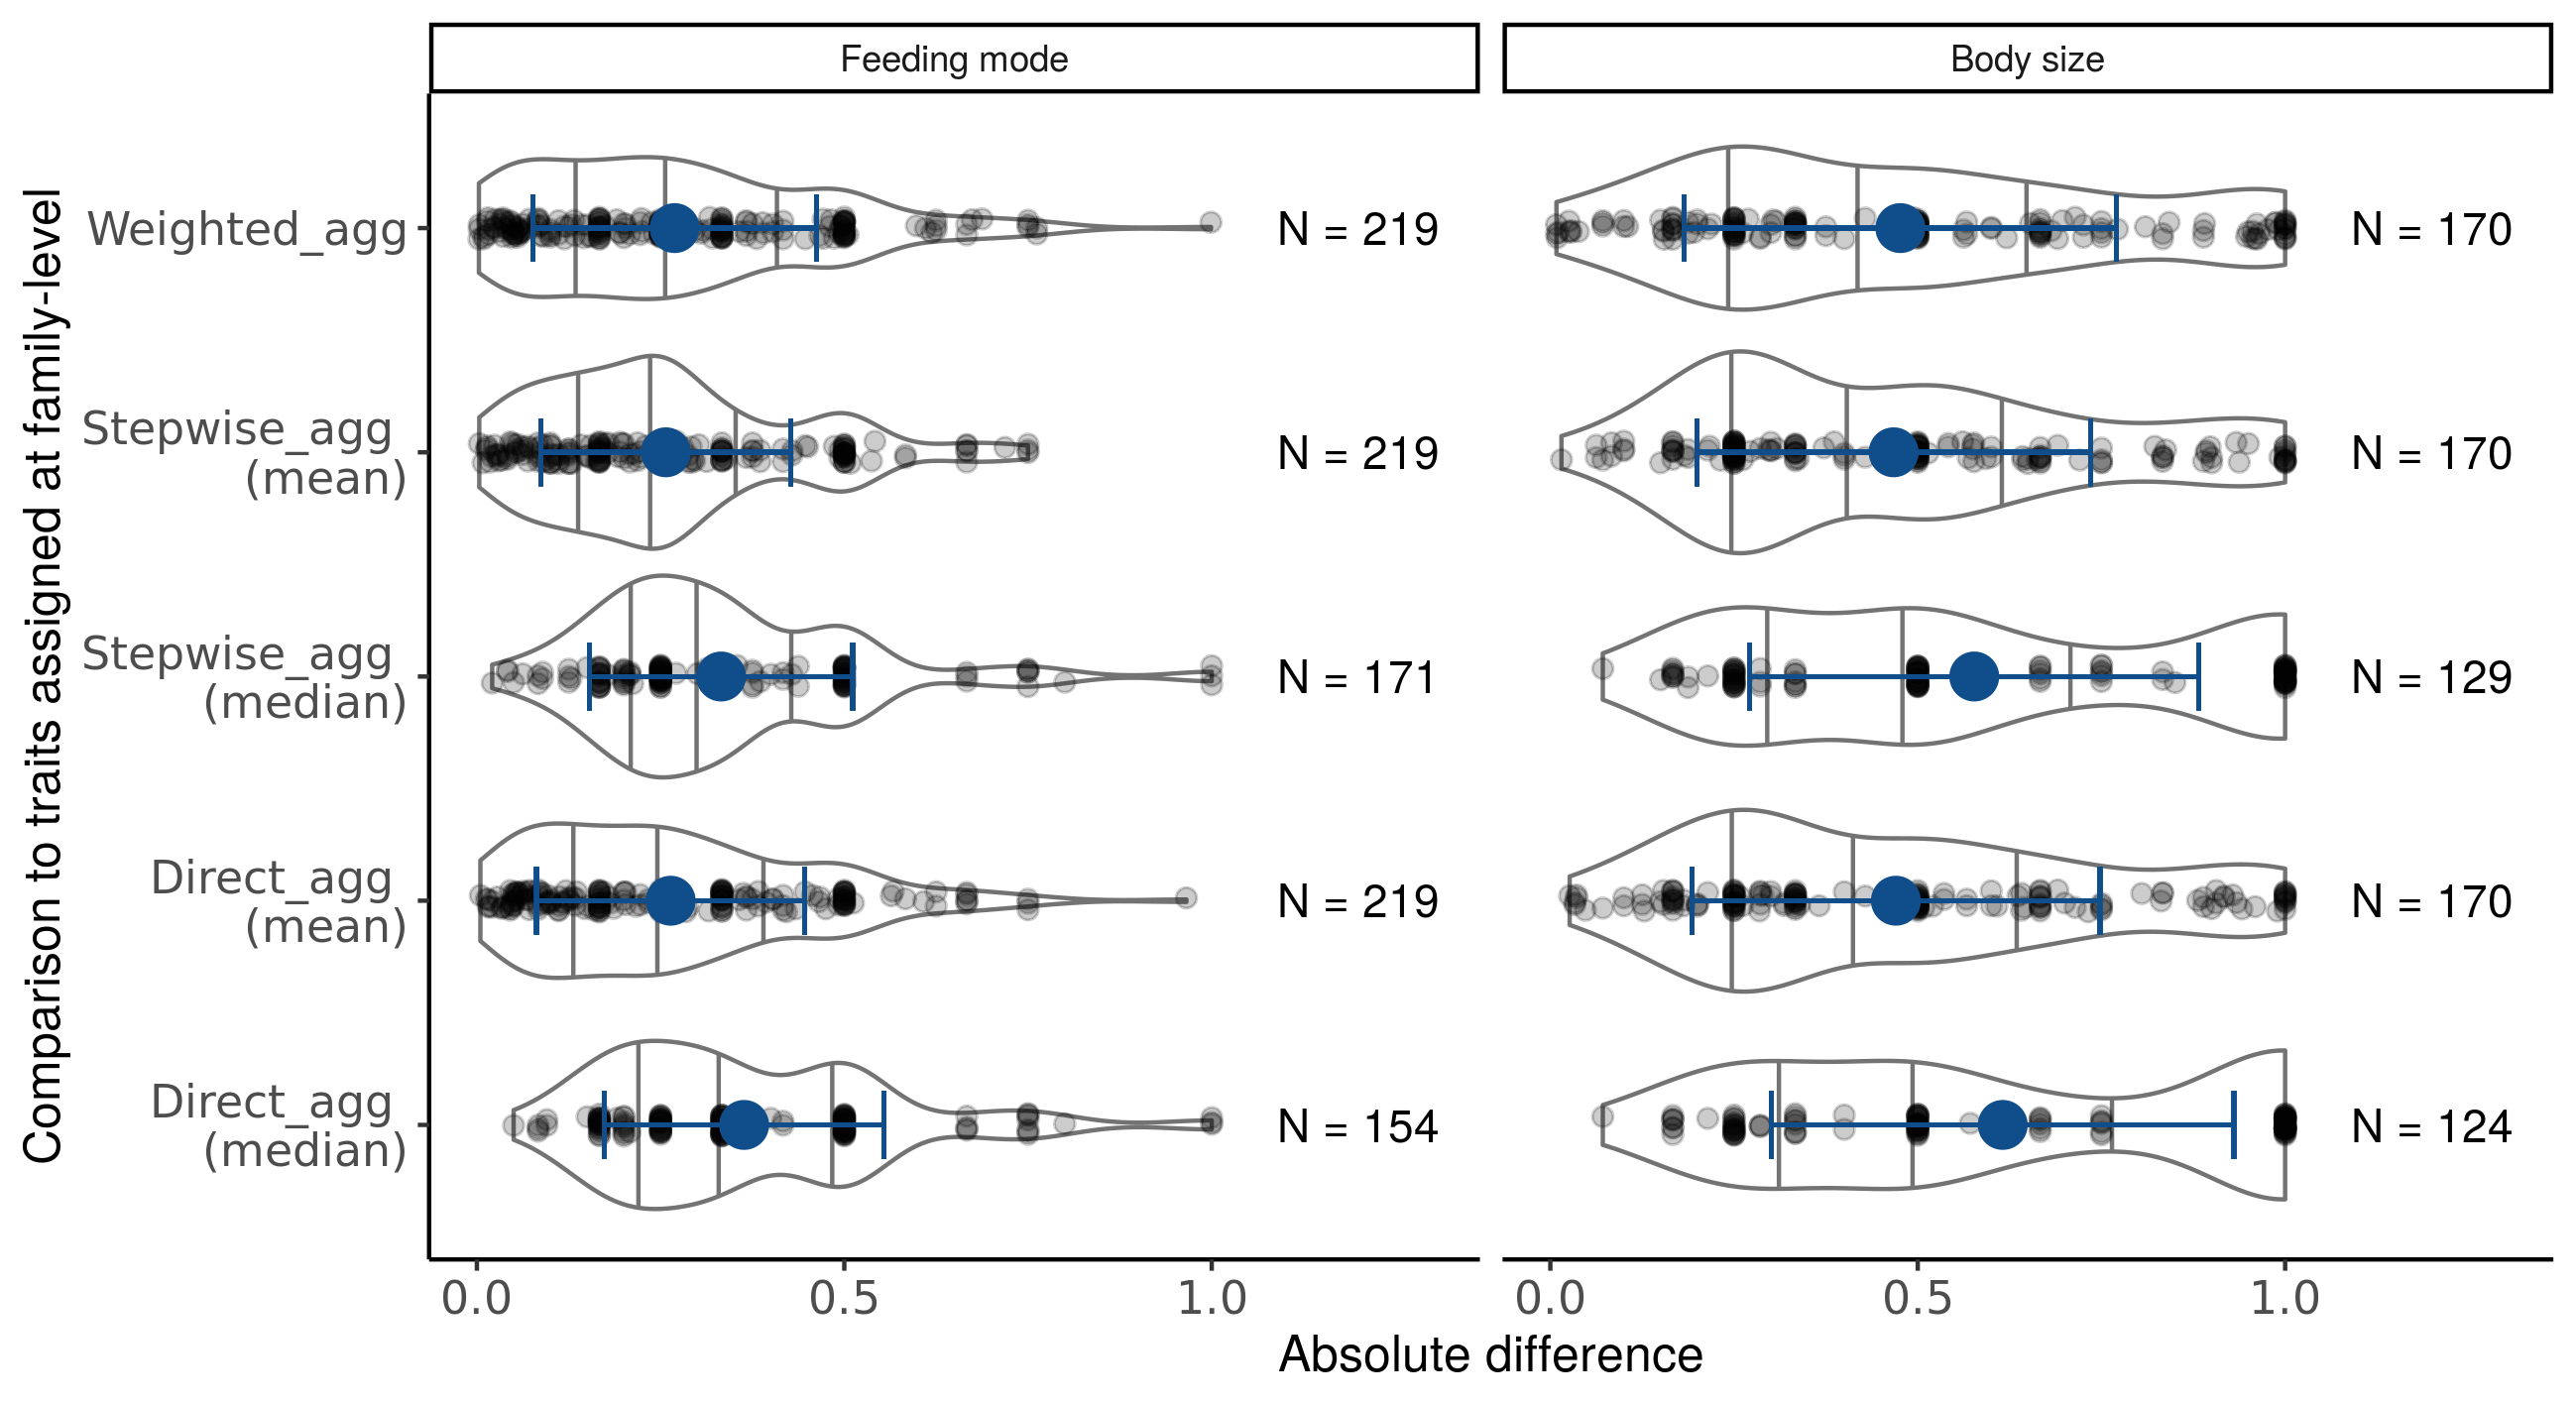
\includegraphics[width=16.5cm, height=10cm]{Deviances_trait_agg_chessman.png}
  \caption{Absolute differences in trait affinities between aggregated traits and traits assigned at family-level by Chessman 2018 for the two grouping features feeding mode and body size. N denotes the number of cases for each comparison. The black dot indicates the mean absolute difference, the error bars the standard deviation. The gray horizontal lines show the 25th, 50th and 75th quantile of the density estimate.}
  \label{fig:diff_aggr_traits_chessman}
\end{figure}


\begin{figure}[H]
  \centering
  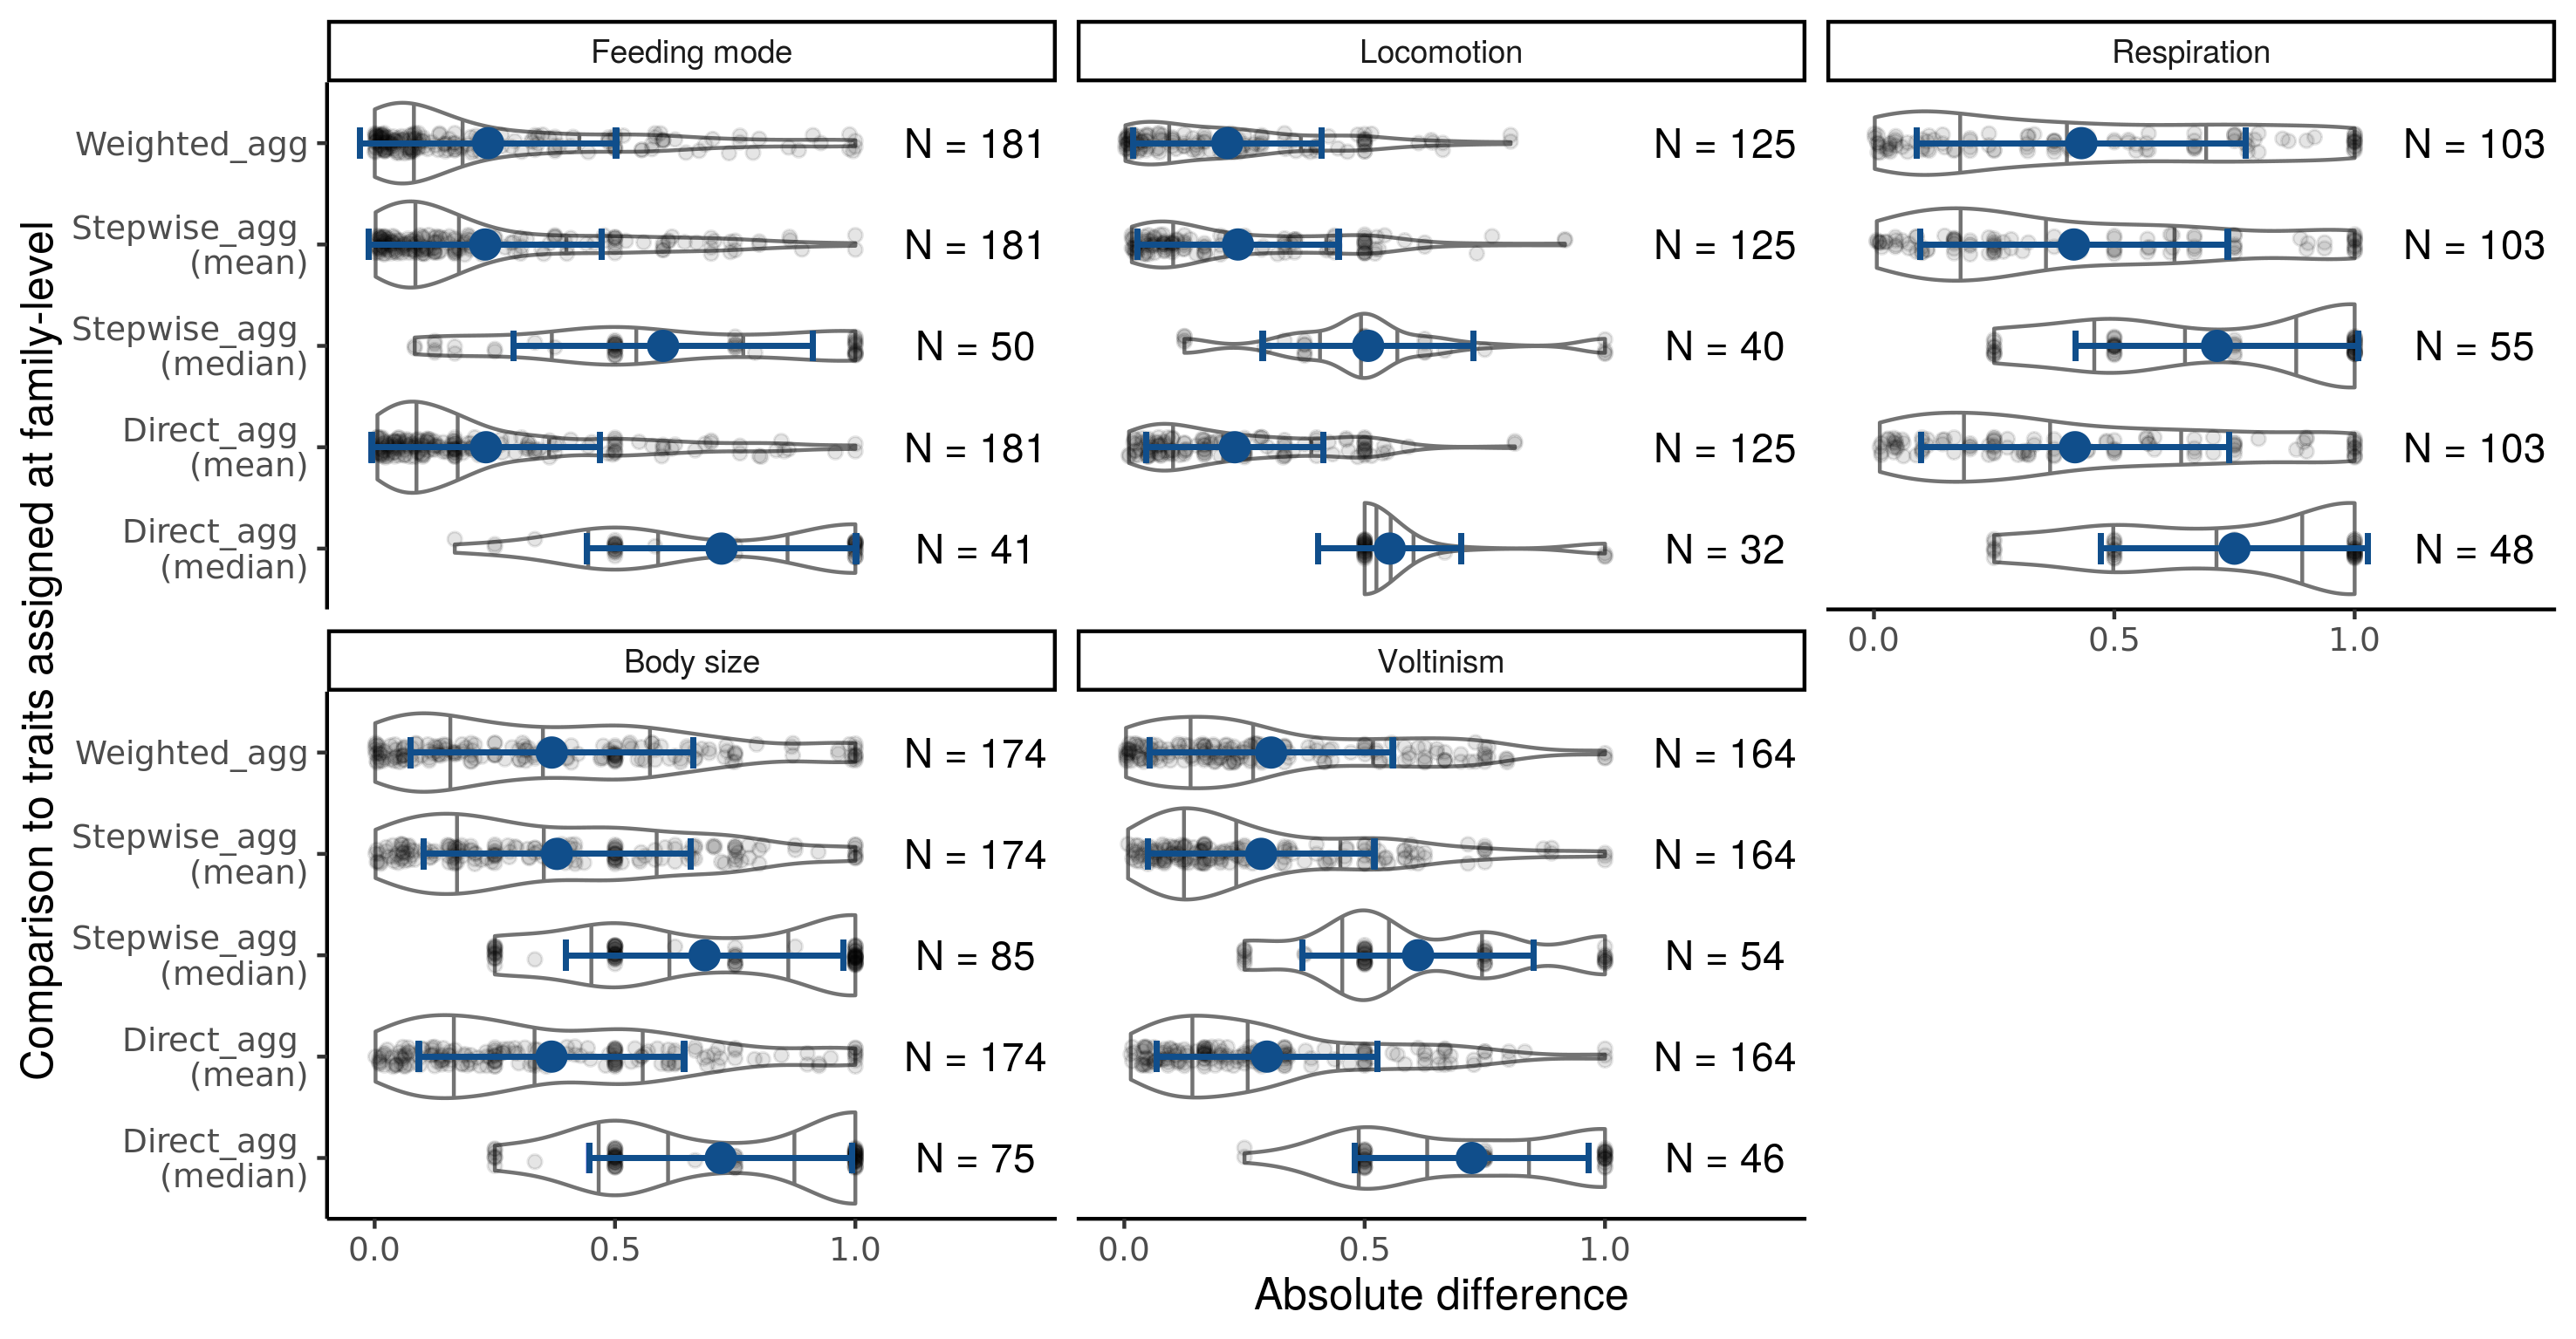
\includegraphics[width=16.5cm, height=10cm]{Deviances_trait_agg_pyne.png}
  \caption{Absolute differences in trait affinities between aggregated traits and traits assigned at family-level by Pyne et al. for the two grouping features feeding mode, locomotion, respiration, body size and voltinism. N denotes the number of cases for each comparison. The black dot indicates the mean absolute difference, the error bars the standard deviation. The gray horizontal lines show the 25th, 50th and 75th quantile of the density estimate.}
  \label{fig:diff_aggr_traits_pyne}
\end{figure}

% \begin{table}[H]
%   \centering
%   \caption{Number of cases per order where trait affinities between \textit{direct\_agg (median)} and \textit{direct\_agg (mean)} compared to at family-level assigned trait affinities by Chessman et al. differed. Penultimate row shows the mean deviance in affinity for deviating cases (standard deviation in parenthesis). Last row shows the mean of absolute deviances in affinities (standard deviation in parenthesis).}
%   \label{tab:direct_agg_vs_chessman}
%   \begin{tabular}{lcc}
%     \hline
%   & \specialcell{Dev. cases \textit{direct\_agg (median)} \\ and family-lvl assigned traits \\ \textit{N = 258}} & \specialcell{Dev. cases \textit{direct\_agg (mean)} \\ and family-lvl assigned traits \\ \textit{N = 354}}\\ 
%   \hline
%   \textbf{Order} &  &  \\ 
%     \textit{Amphipoda} & 17 (6.6\%) & 21 (5.9\%) \\ 
%     \textit{Architaenioglossa} & 2 (0.8\%) & 2 (0.6\%) \\ 
%     \textit{Arhynchobdellida} & 1 (0.4\%) & 1 (0.3\%) \\ 
%     \textit{Coleoptera} & 46 (18\%) & 54 (15\%) \\ 
%     \textit{Collembola} & 6 (2.3\%) & 6 (1.7\%) \\ 
%     \textit{Decapoda} & 8 (3.1\%) & 13 (3.7\%) \\ 
%     \textit{Diptera} & 76 (29\%) & 88 (25\%) \\ 
%     \textit{Ephemeroptera} & 12 (4.7\%) & 19 (5.4\%) \\ 
%     \textit{Hemiptera} & 11 (4.3\%) & 14 (4.0\%) \\ 
%     \textit{Isopoda} & 9 (3.5\%) & 17 (4.8\%) \\ 
%     \textit{Lepidoptera} & 4 (1.6\%) & 5 (1.4\%) \\ 
%     \textit{Lumbriculida} & 0 (0\%) & 2 (0.6\%) \\ 
%     \textit{Mecoptera} & 2 (0.8\%) & 2 (0.6\%) \\ 
%     \textit{Megaloptera} & 2 (0.8\%) & 2 (0.6\%) \\ 
%     \textit{Neuroptera} & 2 (0.8\%) & 2 (0.6\%) \\ 
%     \textit{Odonata} & 4 (1.6\%) & 6 (1.7\%) \\ 
%     \textit{Plecoptera} & 7 (2.7\%) & 16 (4.5\%) \\ 
%     \textit{Rhynchobdellida} & 0 (0\%) & 3 (0.8\%) \\ 
%     \textit{Trichoptera} & 48 (19\%) & 76 (21\%) \\ 
%     \textit{Unionida} & 0 (0\%) & 2 (0.6\%) \\ 
%     \textit{Venerida} & 1 (0.4\%) & 3 (0.8\%) \\ 
%     \hline
%     \textbf{Mean deviances} & -0.018 (0.48) & -0.001 (0.38) \\ 
%     \hline
%     \textbf{Mean abs. deviances} & 0.405 (0.26) & 0.312 (0.21) \\ 
%     \hline
%   \end{tabular}
%   \end{table}

% range  
% than SD and abs mean
% ost of the deviations occurred for both methods for the orders Coleoptera, Diptera and Trichoptera and were in the maximum range possible of 1 to -1. For both methods these deviations occurred for all grouping features (Figure SI \ref{tab:cases_100_direct_agg_pyne}). The standard deviation of the deviating trait affinities for the comparison \textit{direct\_agg (median)} and at family-level assigned trait was 0.62 and the mean of absolute deviances 0.573. The standard deviation of the deviating trait affinities for the comparison \textit{direct\_agg (mean)} and at family-level assigned trait was 0.43 and the mean of absolute deviances 0.346 (Table \ref{tab:weighted_agg_vs_pyne}).

% \begin{table}[H]
%   \centering
%   \caption{Number of cases per order where trait affinities between \textit{direct\_agg (median)} and \textit{direct\_agg (mean)} compared to at family-level assigned trait affinities by Pyne differed. Penultimate row shows the mean deviance in affinity for deviating cases (standard deviation in parenthesis). Last row shows the mean of absolute deviances in affinities (standard deviation in parenthesis).}
%   \label{tab:weighted_agg_vs_pyne}
%   \begin{tabular}{lcc}
%   \hline
%   & \specialcell{Dev. cases \textit{direct\_agg (median)} \\ and family-lvl assigned traits, \\ \textit{N = 273}} & \specialcell{Dev. cases \textit{direct\_agg (mean)} \\ and family-lvl assigned traits, \\ \textit{N = 561}} \\ 
%     \hline
%   \textbf{Order} &  &  \\ 
%     \textit{Coleoptera} & 46 (17\%) & 73 (13\%) \\ 
%     \textit{Diptera} & 53 (19\%) & 109 (19\%) \\ 
%     \textit{Ephemeroptera} & 64 (23\%) & 104 (19\%) \\ 
%     \textit{Hemiptera} & 16 (5.9\%) & 34 (6.1\%) \\ 
%     \textit{Megaloptera} & 4 (1.5\%) & 9 (1.6\%) \\ 
%     \textit{Neuroptera} & 4 (1.5\%) & 4 (0.7\%) \\ 
%     \textit{Odonata} & 12 (4.4\%) & 26 (4.6\%) \\ 
%     \textit{Plecoptera} & 17 (6.2\%) & 57 (10\%) \\ 
%     \textit{Trichoptera} & 57 (21\%) & 145 (26\%) \\ 
%   \hline
%   \textbf{Mean deviances} & -0.029 (0.62) & -0.001 (0.43) \\ 
%   \hline
%   \textbf{Mean abs. deviances} & 0.573 (0.24) & 0.346 (0.26) \\ 
%   \hline
%   \end{tabular}
%   \end{table}




% \begin{figure}[H]
%     \centering
%     \includegraphics[width=16.5cm, height=10cm]{Deviances_dir_median_noa_feed.png}
%     \caption{Deviances in trait affinities for the grouping feature feeding mode for all deviating cases between the \textit{direct\_agg (median)} and assignments at family-level by Pyne et al.}
%     \label{fig:dir_agg_median_feed_pyne}
% \end{figure}

% \begin{figure}[H]
%   \centering
%   \includegraphics[width=16.5cm, height=8cm]{Deviances_dir_median_noa_locom.png}
%   \caption{Deviances in trait affinities for the grouping feature locomotion for all deviating cases between the \textit{direct\_agg (median)} and assignments at family-level by Pyne et al.}
%   \label{fig:dir_agg_median_locom_pyne}
% \end{figure}

% \begin{figure}[H]
%   \centering
%   \includegraphics[width=16.5cm, height=8cm]{Deviances_dir_median_noa_resp.png}
%   \caption{Deviances in trait affinities for the grouping feature respiration for all deviating cases between the \textit{direct\_agg (median)} and assignments at family-level by Pyne et al.}
%   \label{fig:dir_agg_median_resp_pyne}
% \end{figure}

% \begin{figure}[H]
%   \centering
%   \includegraphics[width=16.5cm, height=8cm]{Deviances_dir_median_noa_size.png}
%   \caption{Deviances in trait affinities for the grouping feature size for all deviating cases between the \textit{direct\_agg (median)} and assignments at family-level by Pyne et al.}
%   \label{fig:dir_agg_median_size_pyne}
% \end{figure}

% \begin{figure}[H]
%   \centering
%   \includegraphics[width=16.5cm, height=8cm]{Deviances_dir_median_noa_volt.png}
%   \caption{Deviances in trait affinities for the grouping feature voltinism for all deviating cases between the \textit{direct\_agg (median)} and assignments at family-level by Pyne et al.}
%   \label{fig:dir_agg_median_volt_pyne}
% \end{figure}

%%%%%%%%%%%%%%%%%%%%%%%%%% OLD %%%%%%%%%%%%%%%%%%%%%%%%%%%%%%%%%%%%%%%%%%%%%%%%%%%%%%%
% \subsection{Deviance in trait affinities between \textit{stepwise\_agg} and \textit{direct\_agg (median)}} \label{sec:dev_stepwise_direct_agg}

% The \textit{stepwise\_agg} and \textit{direct\_agg (median)} approaches yielded for the majority of taxa the same affinity (Table \ref{tab:dev_cases_stepwise_median_dir_median}). The amount of cases where the two aggregation methods resulted in different affinities varied between approximately 0.5 \% and 3 \% per database. One case here is a taxa resolved on family-level with a specific trait.

% \begin{table}[H]
%     \centering
%     \caption{Percentage of cases for which the \textit{stepwise\_agg} and \textit{direct\_agg (median)} methods resulted in different trait affinities on family-level. A case is a factor combination of family and trait.}
%     \label{tab:dev_cases_stepwise_median_dir_median}
%     \begin{tabular}{lrr}
%     \hline
%     Database & Deviating cases [\%] & Number of cases \\ 
%     \hline
%     Europe & 1.77 & 2200 \\ 
%       North America & 0.54 & 1300 \\ 
%       Australia & 3.00 & 400 \\ 
%       New Zealand & 1.16 & 1900 \\ 
%     \hline
%     \end{tabular}
%     \end{table}

% Deviances in trait affinities occurred for all grouping features except body form. Deviances ranged between -0.67 (family \textit{Baetidae}, trait herbivore) and 0.6 (family \textit{Libellulidae}, trait size medium). Standard deviations of the deviances varied between databases, i.e. only a small standard deviation in the Australian database (0.09) and relatively large in the North American database (0.43). The mean of the absolute deviances showed that deviances in the North American database, albeit seldom, were high (0.37) and close to zero in the Australian database (0.07) (Table \ref{tab:mean_dev_stepwise_dir}, Figure SI\ref{fig:stepwise_dir_agg}). Deviances in aggregated trait affinities occurred for all investigated grouping features.

% % Cases with differences in trait affinities of more than 30 \% are summarized in table SI\ref{tab:highest_dev_stepwise_dir}. 

% Repeating this analysis with a higher number of taxa using only the three grouping features feeding mode, respiration, and locomotion (Europe = 898, North America = 1033, Australia = 587, New Zealand = 470) resulted in a similar picture. The percentage of deviating cases between \textit{direct\_agg} and \textit{stepwise\_agg} ranged between 1.3 \% (New Zealand) and 4 \% (Europe). 

% As mentioned above, the highest deviance in trait affinity observed was for the family \textit{Baetidae} for the trait herbivore. In this case \textit{stepwise\_agg} was zero and the \textit{direct\_agg (median)} 0.67. Manual examination showed that 7 taxa exist for this family in the European database, 5 of them at species-level and 2 at genus-level. None of the species belonged to the same genus. The affinities of the taxa were the following: (0.9, 0.7, 0, 0.67, 0, 0.75, 0.43). The steps of the \textit{stepwise\_agg} are: I) aggregation to genus-level using the median, which did not change the affinities. II) Subsequent aggregation to family-level using the mode, which resulted in the trait herbivore being assigned affinity 0. The \textit{direct\_agg} results in a more realistic affinity in this case (0.67). 
% % The differences for \textit{Libellulidae} for the traits size large and medium in the European database can be explained in the same way. 

% In general, both methods seem to yield similar trait affinities. Furthermore, using the mode within the \textit{stepwise\_agg} seems to produce rather unrealistic affinities in some scenarios. Hence, we limit our analysis in the following sections to the \textit{direct\_agg} and \textit{weighted\_agg}.

% \begin{table}[H]
%   \centering
%   \caption{Number of cases per order where affinities between \textit{stepwise\_agg} and \textit{direct\_agg} differed per database. Penultimate row shows the mean deviance in affinity for deviating cases (standard deviation in parenthesis). Last row shows the mean of absolute deviances in affinities (standard deviation in parenthesis).}
%   \label{tab:mean_dev_stepwise_dir}
%   \begin{tabular}{lllll}
%   \hline
%   & \specialcell{Australia \\ (\textit{N = 12)}} & \specialcell{Europe \\ (\textit{N = 39})} & \specialcell{New Zealand \\ (\textit{N = 22})} & \specialcell{North America \\ (\textit{N = 7})} \\ 
%     \hline
%   \textbf{Order} &  &  &  &  \\ 
%     \textit{Coleoptera} & 0 (0\%) & 0 (0\%) & 4 (18\%) & 0 (0\%) \\ 
%     \textit{Diptera} & 0 (0\%) & 6 (15\%) & 5 (23\%) & 0 (0\%) \\ 
%     \textit{Ephemeroptera} & 0 (0\%) & 4 (10\%) & 0 (0\%) & 2 (29\%) \\ 
%     \textit{Odonata} & 0 (0\%) & 9 (23\%) & 0 (0\%) & 0 (0\%) \\ 
%     \textit{Onychura} & 0 (0\%) & 0 (0\%) & 0 (0\%) & 2 (29\%) \\ 
%     \textit{Plecoptera} & 8 (67\%) & 8 (21\%) & 2 (9.1\%) & 0 (0\%) \\ 
%     \textit{Spinicaudata} & 0 (0\%) & 0 (0\%) & 0 (0\%) & 2 (29\%) \\ 
%     \textit{Trichoptera} & 4 (33\%) & 12 (31\%) & 11 (50\%) & 1 (14\%) \\ 
%     \hline
%     \textbf{Mean dev.} & 0.049 (0.09) & -0.037 (0.27) & -0.053 (0.17) & 0.012 (0.43) \\
%     \hline 
%     \textbf{Mean abs. dev.} & 0.07 (0.07) & 0.22 (0.16) & 0.15 (0.10) & 0.37 (0.17)
%     \\
%     \hline
%   \end{tabular}
%   \end{table}

% % \begin{table}[H]
% %   \centering
% %   \caption{Cases where affinities of the \textit{stepwise\_agg} and 
% %   \textit{direct\_agg} differed for more than 30 \%.}
% %   \label{tab:highest_dev_stepwise_dir}
% %   \begin{tabular}{llllccc}
% %     \hline
% %     Database & Trait & Order & Family & \specialcell{Affinity \\ \textit{stepwise\_agg}} & \specialcell{Affinity \\ \textit{direct\_agg}} & \specialcell[c]{Deviance \\ in affinity} \\ 
% %     \hline
% %   Europe & feed\_herbivore & Ephemeroptera & Baetidae & 0.00 & 0.67 & -0.67 \\ 
% %     Europe & size\_medium & Diptera & Ceratopogonidae & 0.00 & 0.30 & -0.30 \\ 
% %     Europe & size\_small & Diptera & Ceratopogonidae & 1.00 & 0.70 & 0.30 \\ 
% %     Europe & size\_large & Odonata & Libellulidae & 0.00 & 0.60 & -0.60 \\ 
% %     Europe & size\_medium & Odonata & Libellulidae & 1.00 & 0.40 & 0.60 \\ 
% %     Europe & size\_large & Plecoptera & Perlidae & 1.00 & 0.62 & 0.38 \\ 
% %     Europe & size\_medium & Plecoptera & Perlidae & 0.00 & 0.38 & -0.38 \\ 
% %     Europe & volt\_semi & Plecoptera & Perlodidae & 1.00 & 0.50 & 0.50 \\ 
% %     Europe & size\_large & Trichoptera & Phryganeidae & 1.00 & 0.68 & 0.32 \\ 
% %     Europe & size\_medium & Trichoptera & Phryganeidae & 0.00 & 0.33 & -0.33 \\ 
% %     New Zealand & feed\_shredder & Trichoptera & Leptoceridae & 0.50 & 1.00 & -0.50 \\ 
% %     North America & size\_medium & Spinicaudata & Limnadiidae & 0.50 & 0.00 & 0.50 \\ 
% %     North America & size\_small & Spinicaudata & Limnadiidae & 0.50 & 1.00 & -0.50 \\ 
% %     North America & size\_medium & Onychura & Lynceidae & 0.50 & 0.00 & 0.50 \\ 
% %     North America & size\_small & Onychura & Lynceidae & 0.50 & 1.00 & -0.50 \\ 
% %     \hline
% %   \end{tabular}
% %   \end{table}

% %%%%%%%%%%%%%%%%%%%%%%%%%%%%%%%%%%%%%%%%%%%%%%%%%%%%%%%%%%%%%%%%%%%%%%%%%%%%%%%%%%%%%%%%%%%%%%%%%%%
% %%%%%%%%%%%%%%%%%%%%%%%%%%%%%%%%%%%%%%%%%%%%%%%%%%%%%%%%%%%%%%%%%%%%%%%%%%%%%%%%%%%%%%%%%%%%%%%%%%%
% \subsection{Comparison of trait affinity values \textit{direct\_agg} using median or mean} 
% \label{sec:comp_direct_agg_median_mean}

% The comparison of the \textit{direct\_agg (median)} with the \textit{direct\_agg (mean)} yielded between 2.23 \% (North America) to 17.05 \% (Europe) deviating cases (Table \ref{tab:dev_dir_agg_mean_median}). 
% Deviations between trait affinities were in a range of -0.4 (family \textit{Gripopterygidae}, trait size small) to 0.48 (family \textit{Gripopterygidae}, trait size medium).
% Most deviations were small as the standard deviation of the deviances were close to 0.1 and the mean of the absolute deviances were close to 0 (Table \ref{tab:mean_dev_dir_median_mean}, see also figure SI\ref{fig:dir_agg_median_mean}). Deviances in aggregated trait affinities occurred for all investigated grouping features.

% \begin{table}[H]
%   \centering
%   \caption{Percentage of cases for which the comparison of \textit{direct\_agg (median)} to \textit{direct\_agg (mean)} resulted in different trait affinities.}
%   \label{tab:dev_dir_agg_mean_median}
%   \begin{tabular}{lrr}
%   \hline
%   Database & Deviating cases [\%] & Number of cases \\ 
%   \hline
%   Europe & 17.05 & 2200 \\ 
%   North America & 2.23 & 1300 \\ 
%   Australia & 6.75 & 400 \\ 
%   New Zealand & 7.16 & 1900 \\ 
%   \hline
%   \end{tabular}
% \end{table}

% \begin{table}[H]
%     \centering
%     \caption{Number of cases per order where affinities between \textit{direct\_agg (median)} and \textit{direct\_agg (mean)} differed per database. Penultimate row shows the mean deviance in affinity for deviating cases (standard deviation in parenthesis). Last row shows the mean of absolute deviances in affinities (standard deviation in parenthesis). Where the taxa were unranked on order-level, the class is displayed.}
%     \label{tab:mean_dev_dir_median_mean}
%     \begin{tabular}{lllll}
%       \hline
%       & \specialcell{Australia \\ (\textit{N = 27)}} & \specialcell{Europe \\ (\textit{N = 375})} & \specialcell{New Zealand \\ (\textit{N = 136})} & \specialcell{North America \\ (\textit{N = 29})} \\ 
%       \hline
%       \textbf{Order or higher} &  &  &  &  \\ 
%       \textit{Amphipoda} & 0 (0\%) & 12 (3.2\%) & 0 (0\%) & 0 (0\%) \\ 
%       \textit{Branchiopoda} & 0 (0\%) & 0 (0\%) & 0 (0\%) & 2 (6.9\%) \\ 
%       \textit{Coleoptera} & 0 (0\%) & 58 (15\%) & 20 (15\%) & 0 (0\%) \\ 
%       \textit{Diptera} & 0 (0\%) & 20 (5.3\%) & 24 (18\%) & 0 (0\%) \\ 
%       \textit{Ephemeroptera} & 0 (0\%) & 41 (11\%) & 11 (8.1\%) & 4 (14\%) \\ 
%       \textit{Gastropoda} & 0 (0\%) & 0 (0\%) & 0 (0\%) & 3 (10\%) \\ 
%       \textit{Hemiptera} & 0 (0\%) & 14 (3.7\%) & 0 (0\%) & 2 (6.9\%) \\ 
%       \textit{Littorinimorpha} & 0 (0\%) & 0 (0\%) & 0 (0\%) & 2 (6.9\%) \\ 
%       \textit{Mollusca} & 0 (0\%) & 0 (0\%) & 8 (5.9\%) & 0 (0\%) \\ 
%       \textit{Odonata} & 0 (0\%) & 56 (15\%) & 5 (3.7\%) & 0 (0\%) \\ 
%       \textit{Onychura} & 0 (0\%) & 0 (0\%) & 0 (0\%) & 2 (6.9\%) \\ 
%       \textit{Plecoptera} & 7 (26\%) & 60 (16\%) & 24 (18\%) & 2 (6.9\%) \\ 
%       \textit{Spinicaudata} & 0 (0\%) & 0 (0\%) & 0 (0\%) & 2 (6.9\%) \\ 
%       \textit{Trichoptera} & 20 (74\%) & 114 (30\%) & 44 (32\%) & 10 (34\%) \\ 
%       \hline
%       \textbf{Mean dev.} & -0.024 (0.08) & -0.008 (0.12) & -0.016 (0.15) & -0.009 (0.16) \\ 
%       \hline
%       \textbf{Mean abs. dev.} & 0.06 (0.05) & 0.09 (0.07) & 0.11 (0.11) & 0.14 (0.08) \\ 
%     \hline
%   \end{tabular}
% \end{table}


% %%%%%%%%%%%%%%%%%%%%%%%%%%%%%%%%%%%%%%%%%%%%%%%%%%%%%%%%%%%%%%%%%%%%%%%%%%%%%%%%%%%%%%%%%%%%%%%%%%%
% %%%%%%%%%%%%%%%%%%%%%%%%%%%%%%%%%%%%%%%%%%%%%%%%%%%%%%%%%%%%%%%%%%%%%%%%%%%%%%%%%%%%%%%%%%%%%%%%%%%
% \subsection{Deviances in trait affinity values between \textit{direct\_agg} and \textit{weighted\_agg}}
% \label{sec:dev_dir_agg_weighted}

% Comparison of the \textit{direct\_agg (median)} with the \textit{weighted\_agg} showed varying levels of cases with deviating trait affinities across databases (between 3.46 \% deviating cases for the North American database up to 19.27 \% in the European database, Table \ref{tab:dev_dir_agg_mean_median}). Likewise, the number of deviating cases varied for the comparison of the \textit{direct\_agg (mean)} with \textit{weighted\_agg}, but was generally lower (between no deviating case for New Zealand and 11.59 \% for the European database). Actually, there were a small number of deviating cases for the New Zealand database. However, the deviances were extremely small (below the 10th decimal place). Hence, we neglected these small deviations. The absence of deviating cases and the similar amount of deviating cases for the comparison \textit{direct\_agg (median)} and \textit{weighted\_agg} to the comparison \textit{direct\_agg (median)} with \textit{direct\_agg (mean)} (Section \ref{sec:comp_direct_agg_median_mean}) for New Zealand reflects the fact that most entries in this database contain complete trait profiles.

% Deviances in trait affinities occurred for both comparisons for all investigated grouping features. Also, for both comparisons deviations between trait affinities were in range of -0.49 (European database, family \textit{Leuctridae}, trait crawler and trait semivoltine) to 0.49 ((European database, family \textit{Leuctridae}, trait burrower). Standard deviations of the deviances between \textit{direct\_agg (median)} and \textit{weighted\_agg} ranged from 0.09 (Australia) to 0.16 (North America). The mean of absolute deviances ranged between 0.068 (Australia) to 0.135 (North America) (Table \ref{tab:mean_dev_median_weighted}). Standard deviations of the deviances between \textit{direct\_agg (mean)} and \textit{weighted\_agg} were smaller and ranged between 0.06 (Australia) and 0.11 (North America), while the mean of absolute deviances were close to zero for all databases (from 0.037 Australia to 0.078 North America) (Table \ref{tab:mean_dev_mean_weighted}, see also figure SI \ref{fig:dir_agg_median_mean_weighted}).

% \begin{table}[H]
%     \centering
%     \caption{Percentage of cases for which \textit{direct\_agg (median)} and \textit{weighted\_agg} resulted in different trait affinities and cases for which \textit{direct\_agg (mean)} and \textit{weighted\_agg} resulted in different trait affinities.}
%     \label{tab:dev_dir_agg_weighted}
%     \begin{tabular}{lccc}
%     \hline
%     Database & \specialcell{Deviating cases \textit{direct\_agg (median)} \\ vs. \textit{weighted\_agg} [\%]} & \specialcell{Deviating cases \textit{direct\_agg (mean)}\\ vs. \textit{weighted\_agg} [\%]} & Nr. of cases \\ 
%     \hline
%     Europe & 19.27 & 11.59 & 2200 \\ 
%     North America & 3.46 & 2.62 & 1300 \\ 
%     Australia & 9.75 & 9.75 & 400 \\ 
%     New Zealand & 7.21 & 0 & 1900 \\ 
%     \hline
%     \end{tabular}
% \end{table}

% \begin{table}[H]
%   \centering
%   \caption{Number of cases per order where affinities between \textit{direct\_agg (median)} and \textit{weighted\_agg} differed per database. Penultimate row shows the mean deviance in affinity for deviating cases (standard deviation in parenthesis). Last row shows the mean of absolute deviances in affinities (standard deviation in parenthesis). If taxa were unranked on order-level, the class is displayed.}
%     \label{tab:mean_dev_median_weighted}
%   \begin{tabular}{lllll}
%     \hline
%     & \specialcell{Australia \\ \textit{N = 39}} & \specialcell{Europe \\ \textit{N = 423}} & \specialcell{New Zealand \\ \textit{N = 137}} & \specialcell{North America \\ \textit{N = 45}} \\ 
%     \hline
%   \textbf{Order or higher} &  &  &  &  \\ 
%     \textit{Amphipoda} & 0 (0\%) & 12 (2.8\%) & 0 (0\%) & 0 (0\%) \\ 
%     \textit{Branchiopoda} & 0 (0\%) & 0 (0\%) & 0 (0\%) & 2 (4.4\%) \\ 
%     \textit{Coleoptera} & 0 (0\%) & 58 (14\%) & 20 (15\%) & 0 (0\%) \\ 
%     \textit{Diptera} & 0 (0\%) & 21 (5.0\%) & 24 (18\%) & 0 (0\%) \\ 
%     \textit{Ephemeroptera} & 0 (0\%) & 60 (14\%) & 11 (8.0\%) & 8 (18\%) \\ 
%     \textit{Gastropoda} & 0 (0\%) & 0 (0\%) & 0 (0\%) & 3 (6.7\%) \\ 
%     \textit{Hemiptera} & 0 (0\%) & 14 (3.3\%) & 0 (0\%) & 3 (6.7\%) \\ 
%     \textit{Littorinimorpha} & 0 (0\%) & 0 (0\%) & 0 (0\%) & 2 (4.4\%) \\ 
%     \textit{Mollusca} & 0 (0\%) & 0 (0\%) & 8 (5.8\%) & 0 (0\%) \\ 
%     \textit{Odonata} & 0 (0\%) & 57 (13\%) & 5 (3.6\%) & 0 (0\%) \\ 
%     \textit{Onychura} & 0 (0\%) & 0 (0\%) & 0 (0\%) & 2 (4.4\%) \\ 
%     \textit{Plecoptera} & 8 (21\%) & 73 (17\%) & 24 (18\%) & 4 (8.9\%) \\ 
%     \textit{Spinicaudata} & 0 (0\%) & 0 (0\%) & 0 (0\%) & 2 (4.4\%) \\ 
%     \textit{Trichoptera} & 31 (79\%) & 128 (30\%) & 45 (33\%) & 19 (42\%) \\
%     \hline 
%     \textbf{Mean deviance} & -0.017 (0.09) & -0.007 (0.13) & -0.016 (0.15) & -0.006 (0.16) \\ 
%     \hline
%     \textbf{Mean abs. deviances} & 0.068 (0.07) & 0.094 (0.09) & 0.112 (0.11) & 0.135 (0.08) \\ 
%   \hline
%   \end{tabular}
%   \end{table}

% \begin{table}[H]
%       \centering
%     \caption{Number of cases per order where affinities between \textit{direct\_agg (mean)} and \textit{weighted\_agg} differed per database. There were no deviating cases for the New Zealand database. Penultimate row shows the mean deviance in affinity for deviating cases (standard deviation in parenthesis). Last row shows the mean of absolute deviances in affinities (standard deviation in parenthesis). If taxa were unranked on order-level, the class is displayed.}
%     \label{tab:mean_dev_mean_weighted}
%     \begin{tabular}{llll}
%     \hline
%     & \specialcell{Australia \\ \textit{N = 39}} & \specialcell{Europe \\ \textit{N = 255}} & \specialcell{North America \\ \textit{N = 34}} \\ 
%     \hline
%     \textbf{Order or higher} &  &  &  \\ 
%       \textit{Amphipoda} & 0 (0\%) & 1 (0.4\%) & 0 (0\%) \\ 
%       \textit{Coleoptera} & 0 (0\%) & 18 (7.1\%) & 0 (0\%) \\ 
%       \textit{Diptera} & 0 (0\%) & 2 (0.8\%) & 0 (0\%) \\ 
%       \textit{Ephemeroptera} & 0 (0\%) & 51 (20\%) & 8 (24\%) \\ 
%       \textit{Hemiptera} & 0 (0\%) & 14 (5.5\%) & 3 (8.8\%) \\ 
%       \textit{Mollusca} & 0 (0\%) & 0 (0\%) & 0 (0\%) \\ 
%       \textit{Odonata} & 0 (0\%) & 28 (11\%) & 0 (0\%) \\ 
%       \textit{Plecoptera} & 8 (21\%) & 40 (16\%) & 4 (12\%) \\ 
%       \textit{Trichoptera} & 31 (79\%) & 101 (40\%) & 19 (56\%) \\ 
%       \hline
%       \textbf{Mean deviance} & 0 (0.06) & 0 (0.08) & 0 (0.11) \\ 
%       \hline
%       \textbf{Mean abs. deviances} & 0.037 (0.04) & 0.041 (0.07) & 0.078 (0.08) \\ 
%       \hline
%       \end{tabular}
% \end{table}


\end{document}